Google Glass, or simply ``Glass'' as the device is known within Google, is a head-mounted display (HMD)\footnote{See section \ref{subsubsec:hmd}.} that can be seen as an augmented reality device\footnote{See section \ref{subsubsec:ar}.} designed to bring notifications to the user more easily than a smartphone does. Google Glass can be seen in Figure \ref{GoogleGlassHardware}. According to Google ``Glass is designed to be there when the user needs it and to stay out of the way when the user does not''.\cite{glassDesignPrinciples} Google Glass is meant to give the user relevant information at relevant times.
%\url{https://developers.google.com/glass/design/principles}
\\
	\begin{figure}[ht!]
		\centering
    \subfloat[The user can control Google Glass with the touchpad.]{{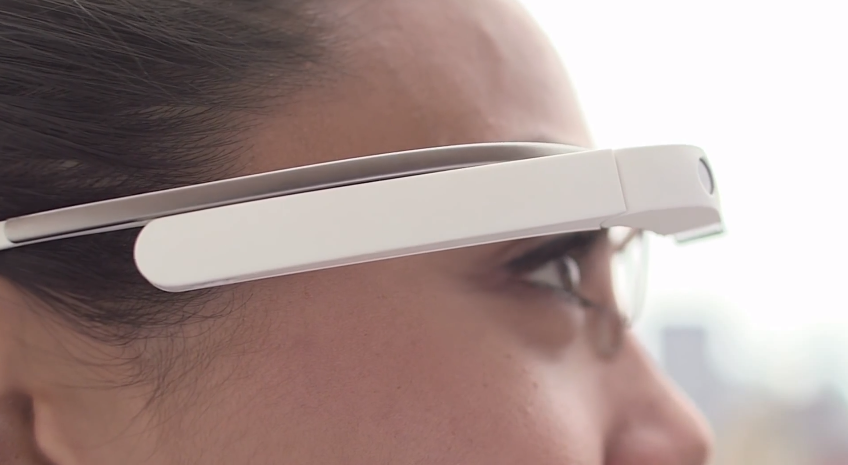
\includegraphics[width=70mm]{images/GoogleGlassHardwareTouchpad} }}
    \qquad
    \subfloat[The display sits slightly above the users line of sight, on the right hand side.]{{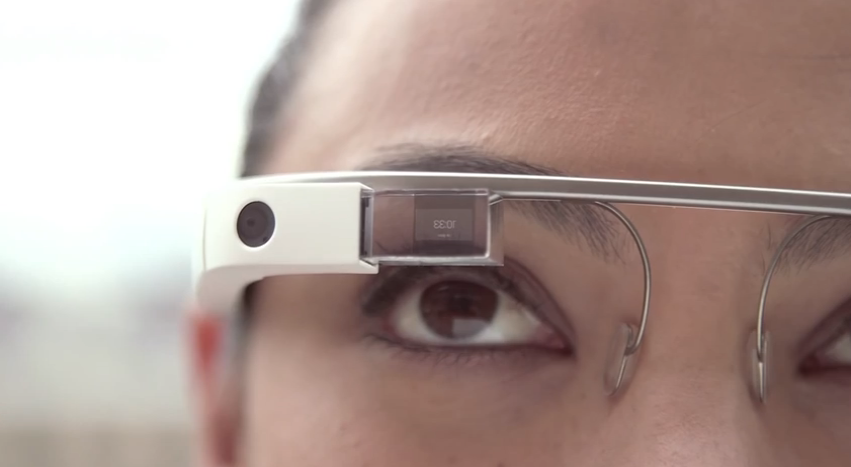
\includegraphics[width=70mm]{images/GoogleGlassHardware} }}
    \qquad
		%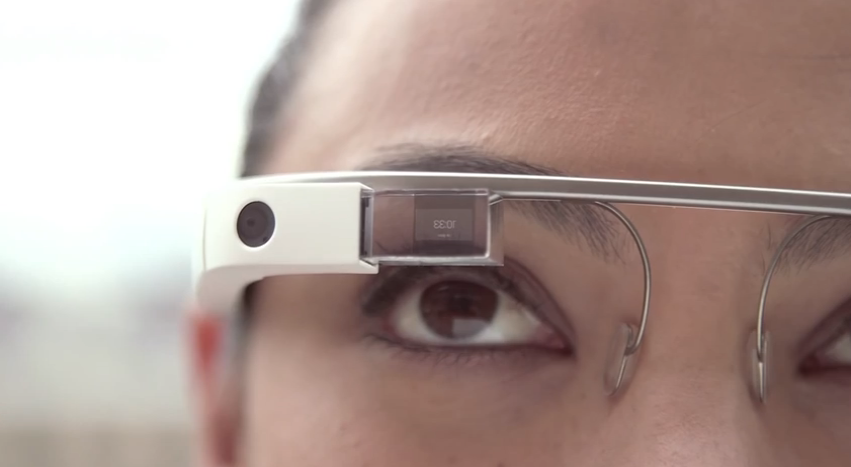
\includegraphics[width=110mm]{images/GoogleGlassHardware}
		\caption{Google Glass is a small head mounted display equipped with a touchpad, a camera and a microphone.\cite{ImagesGoogleGlassUI}}
		\label{GoogleGlassHardware}
	\end{figure}
\\
Google Glass is partially controlled with a touchpad, but can also be controlled through voice commands. The touchpad sits on the right hand side of the user's glass frame and runs from the temple to the ear (see in Figure \ref{GoogleGlassHardware} (a)). When the user touches anywhere on the touchpad Google Glass ``wakes up'' from stand by and displays the start screen (which consists of a clock). The display is mounted above the user's line of sight, on the right hand side (see Figure \ref{GoogleGlassHardware} (b)) and can be slightly adjusted so that the user can see all that is currently being displayed.
\\
\\
The display is a projection that goes through an optic lense in the glass piece, seen in Figure \label{GoogleGlassHardware} (b), which creates a virtual image. A virtual image is an image that, projected through optic lenses, appears to be located at at a point where the actual projection is not.\cite{virtualImageWiki} In the case of Google Glass the display appears to be located further away from the user than the display actually is. The display is said to be equivalent of a 25 inch high definition screen seen from a distance of approximately 2.5 meters.\cite{GlassSpecs}

%
%
%
%
%
%
%
%	\begin{figure}[ht!]
%		\centering
%		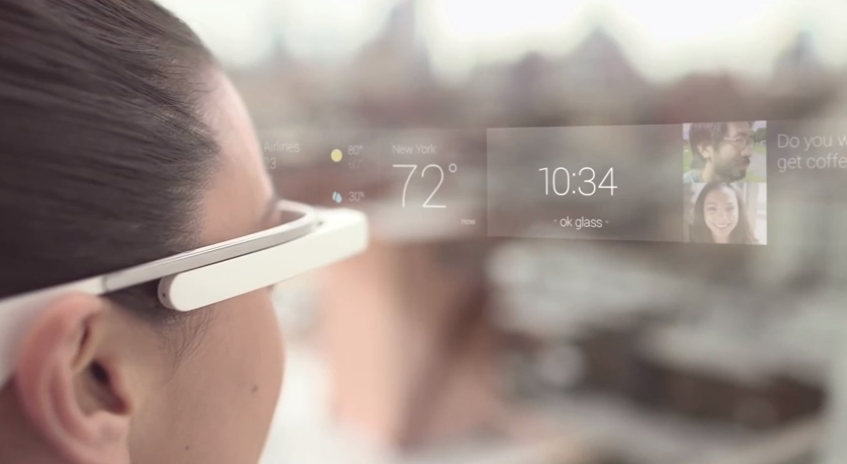
\includegraphics[width=110mm]{images/GoogleGlassUI}
%		\caption{A virtual representation of the Google Glass user interface as the graphical user interface is perceived by the user.\cite{ImagesGoogleGlassUI}}
%		\label{GoogleGlassUI}
%	\end{figure}
%	
%	
%	
%
%
%
%
%The graphical user interface (GUI) is called a timeline (see Figure \ref{GoogleGlassUI}). The timeline consists of a row of cards. Cards are basic applications such as a clock or information about the weather. Cards can also represent more in-depth applications, on Google Glass called ``Immersions''. An immersion handles activities such as browsing an image gallery or playing a game.\\
%
%On the timeline cards to the left of the home screen are upcoming activities such as an event in the user's calendar or an upcoming flight. Cards to the right of the home screen are from the past. Cards from the past will for instance show text messages or photos. When the user wants to turn of Google Glass the user swipes down on the touchpad. Swiping down on the touchpad will put Google Glass in stand by. If the user wants to turn of Google Glass entirely there is a power button on the opposite side of the touchpad. Holding down the power button for a few seconds will turn of Google Glass. For a better visual understanding of how Google Glass works see Figure \ref{GoogleGlassUI} as well as the video referenced in the caption.\\
%
%Glass uses a small display placed to the upper right of the user's line of sight and is mounted on the user as a regular pair of glasses. Equipped with a camera, microphone and speakers it is capable of performing a lot of the tasks users normally would do on a smartphone such as taking photographs, video chatting, writing text messages.
%
%
\subsubsection{Head-Mounted Display (HMD)}
\label{subsubsec:hmd}
A head-mounted display (HMD)\cite{hmdWiki} is a device that is worn on the head and that places a small display in front of one or both of the user's eyes. The device can either be a stand alone device or a part of a helmet. A branch of HMDs are optical head-mounted displays (OHMDs)\cite{ohmdWiki}. A OHMD is a HMD with a see-through display, such as Google Glass.
%A head mounted display is just as it sounds a display that goes on ones head and that displays stuff

\subsubsection{Heads-Up Display (HUD)}
\label{subsubsec:hud}
A heads-up display (HUD)\cite{hudWiki} is defined as any transparent display that, when presenting information, does not require userss to look away from their usual viewpoints. In other words, a HUD may be a HMD and a HMD may be a HUD. While a HMD is always worn on the head a HUD can be a stand-alone display. In contrast a HUD must be a transparent display. A requirement a HMD does not have. A OHMD, however, is always a HUD since a OHMD has a transparent display.

\subsubsection{Virtual Reality}
\label{subsubsec:vr}
Virtual reality\cite{virtualRealityDef} is defined as a computer generated simulation that enables users to interact with a three-dimensional environment. Virtual realities are common in interactive mediums such as video games. Virtual realities can also be combined with a HMD in order to completely engulf the user in the virtual reality. One such example is the Oculus Rift, seen in Figure \ref{OculusRift}, that completely covers the user's eyes, allowing the user to get emerged in the virtual reality.
\\
	\begin{figure}[ht!]
		\centering
		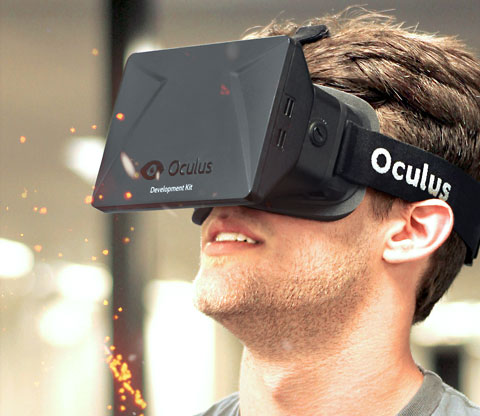
\includegraphics[width=110mm]{images/OculusRift}
		\caption{The virtual reality device ``Oculus Rift'' is a HMD that completely covers the user's eyes.\cite{ImagesOculusRift}}
		\label{OculusRift}
	\end{figure}
\\
Google Glass is able to display a virtual reality but does not work as a virtual reality device. Google Glass only covers a small part of the user's sight and as such does not have the capability of simulating a three-dimensional, interactive, environment in contrast to the Oculus Rift. Oculus Rift, unlike Google Glass, is able to replace the user's reality with a completely virtual reality since Oculus Rift completely covers the user's eyes.

\subsubsection{Augmented Reality}
\label{subsubsec:ar}
Augmented reality\cite{augmentedRealityDef} is defined as the combination of reallty (or what is within current context being perceived as reality\footnote{Augmented reality is for instance common in video games to give the player environmental and health information.}) with useful, computer generated, data. Augmented reality, unlike virtual reality, is not meant to replace reality, but rather to enhance interaction with the current reality.
\\
\\
A HUD may create an augmented reality. The reason a HUD does not always create an augmented reality is due to the fact that the information being presented might not be useful within the current context. An augmented reality is, as stated above, meant to enhance reality, while a HUD does not have that requirement.
\\
\\
Google Glass is a HUD that have the potential (and intent) to create an augmented reality. Google Glass is meant to bring useful information to the user while not distracting from reality. One example of useful information that could enhance the users interaction with reality would be a shopping list while shopping, as seen in Figure \ref{GlassShopping}.
\\
	\begin{figure}[ht!]
		\centering
		
\includegraphics[width=110mm]{images/GoogleGlassKeepRevelant}
		\caption{One way of bringing useful information to the user would be by displaying a shopping list while the user is out shopping.\cite{glassDesignPrinciples}}
		\label{GlassShopping}
	\end{figure}
	
	
%\subsubsection{Augmented Reality vs Virtual Reality}
%\label{subsubsec:augmentedrealityvsvirtualreality}

%[TODO WRITE ABOUT HUD AND HMD]

%When discussing head mounted displays it is possible that the first image that pops into ones head is similar to Figure \ref{OculusRift}. What is important to note about Oculus Rift (Figure \ref{OculusRift}) and other similar product that completely covers the user's eyes is that these are all virtual reality devices. Virtual reality is not the same as augmented reality, which is what Google Glass gives the user.

%The difference lies in how much of what the user can see is computer generated. In a virtual reality the entire environment is computer generated. Augmented reality on the other hand is based in reality where computer generated elements of the environment help enhance reality. In other words: virtual reality replaces reality and augmented reality enhance reality. Since Google Glass does not remove the user from reality but rather display information that can be consumed at the same time as the user experience the real world Google Glass is an augmented reality device compared to Oculus Rift which is a virtual reality device.

%TODO --- ADD HUD vs AUGMENTED REALITY!!!!!!


%What is it?
%Augmented Reality vs Virtual Reality
%Define Augmented Reality
%Define Virtual Reality
